% Test document: renders every delivered float in the layout the paper uses.
\documentclass[twocolumn]{article}
\usepackage[margin=0.75in]{geometry}
\usepackage{booktabs,graphicx,amsmath,amssymb,pifont,xspace,caption,subcaption}
\usepackage[table]{xcolor}
\newcommand{\model}{\texttt{\textsc{VL-Rethinker}}\xspace}
\graphicspath{{../}}
\begin{document}
\begin{figure*}[tb]
\centering
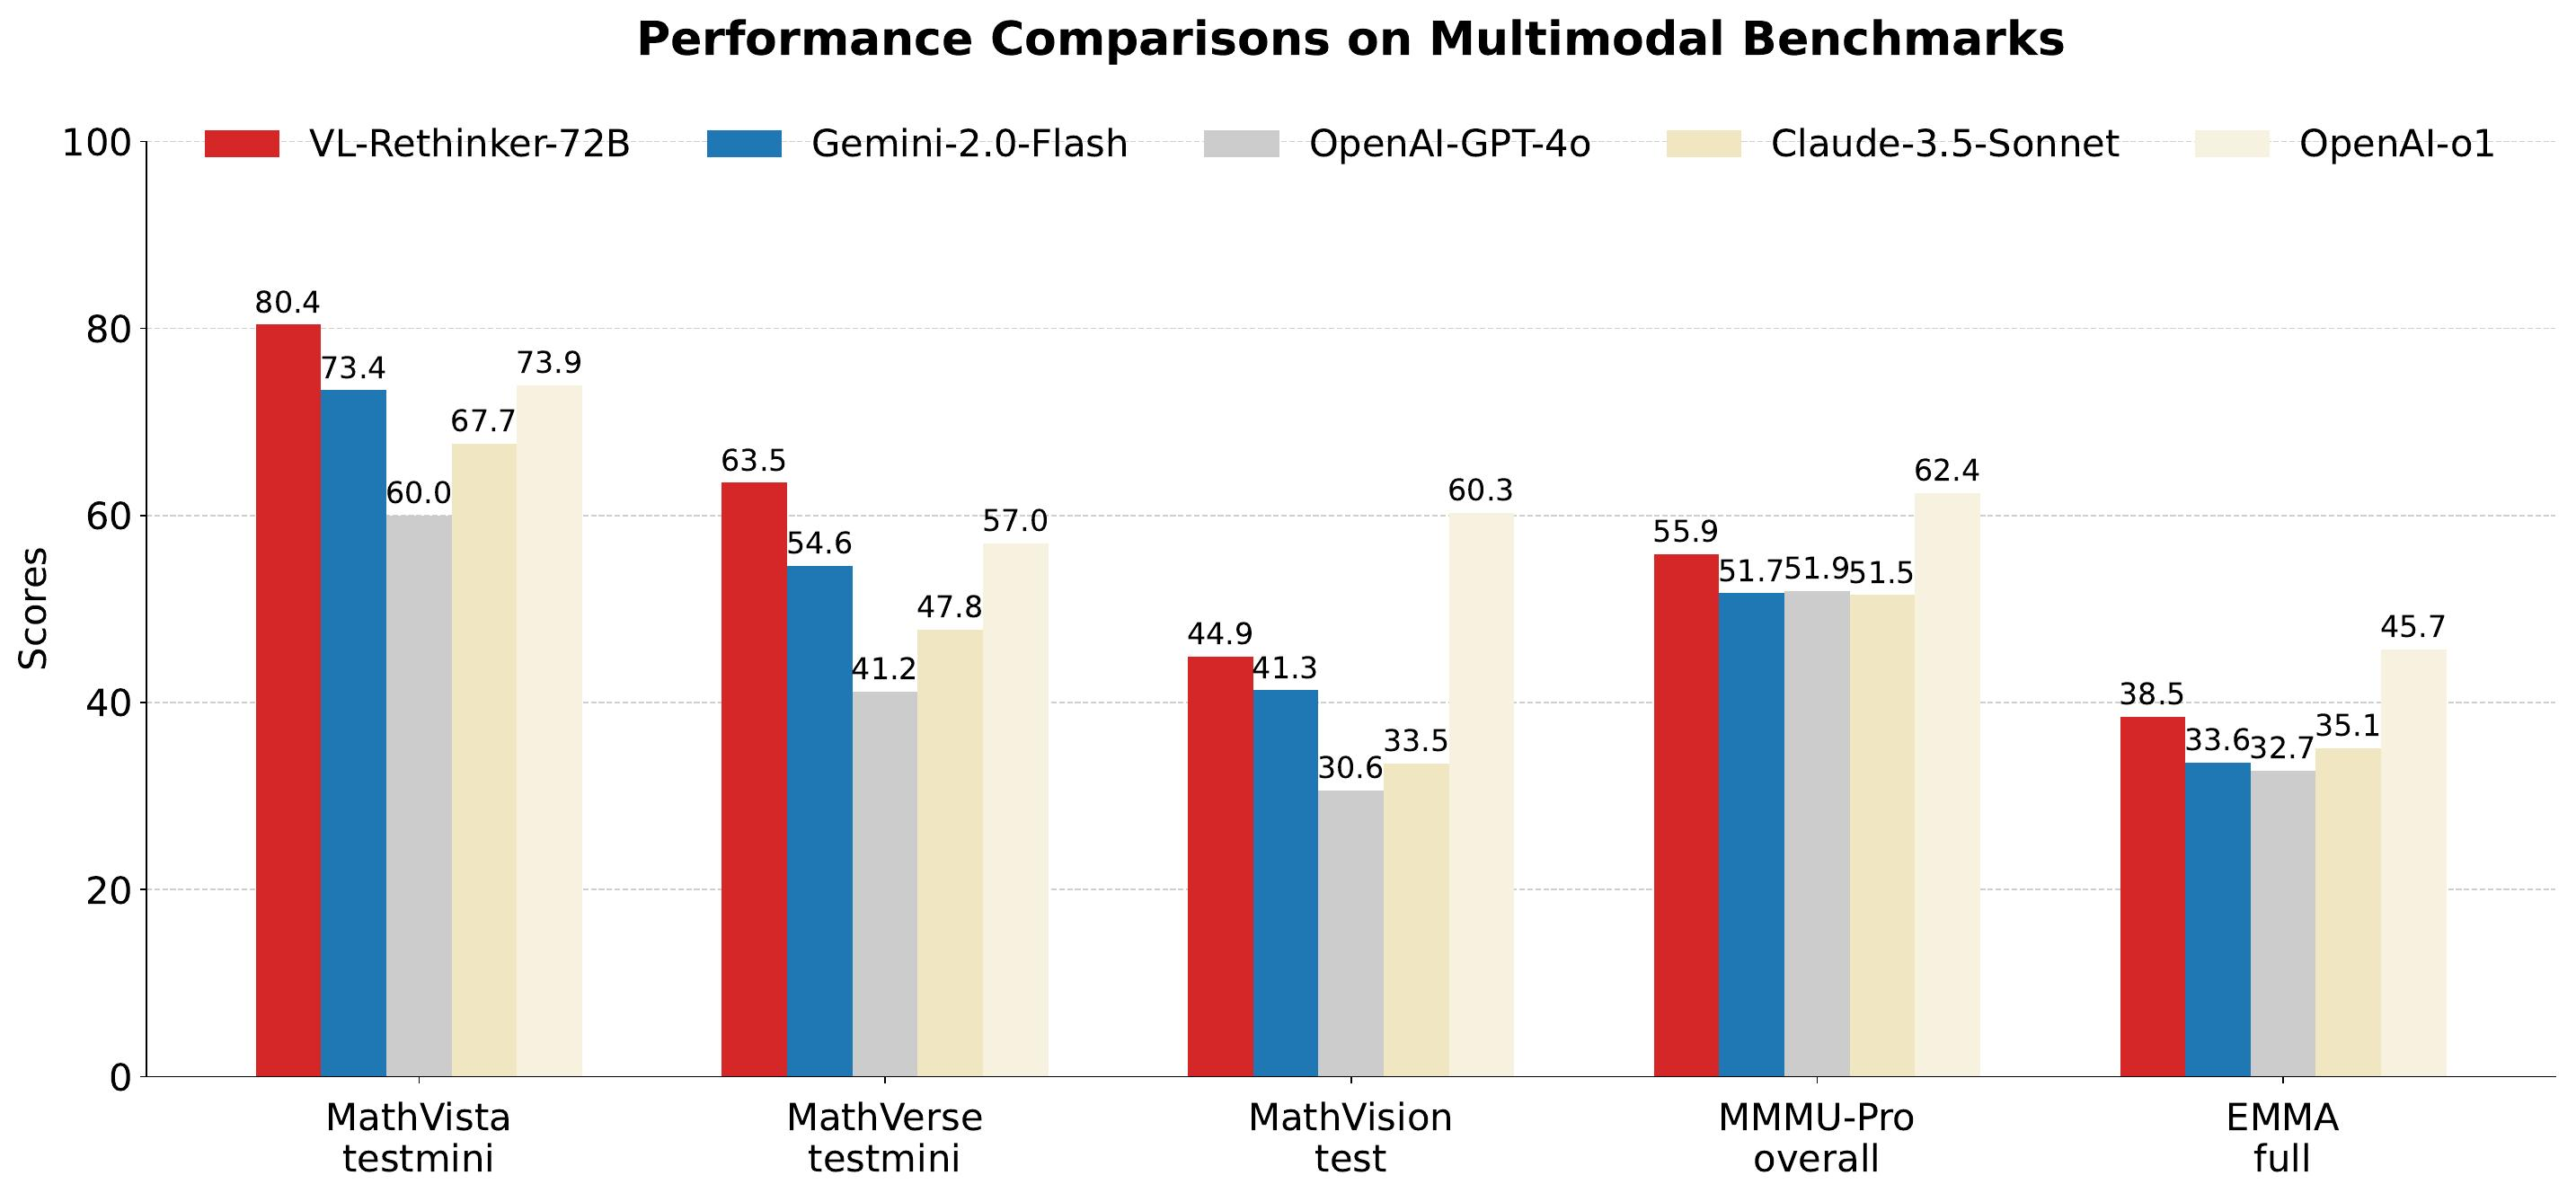
\includegraphics[width=\textwidth]{figures/teaser-2.jpg}
\caption{\small \textbf{\model-72B compared with proprietary models.} Accuracy (\%) on MathVista testmini, MathVerse testmini, MathVision test, MMMU-Pro overall and EMMA full (values as in Table~\ref{table:main_results}). \model-72B scores higher than GPT-4o, Claude-3.5-Sonnet and Gemini-2.0-Flash on all five benchmarks and higher than OpenAI-o1 on MathVista and MathVerse; o1 remains ahead on MathVision, MMMU-Pro and EMMA.}
\label{fig:teaser}
\end{figure*}

\begin{figure*}[tb]
\centering
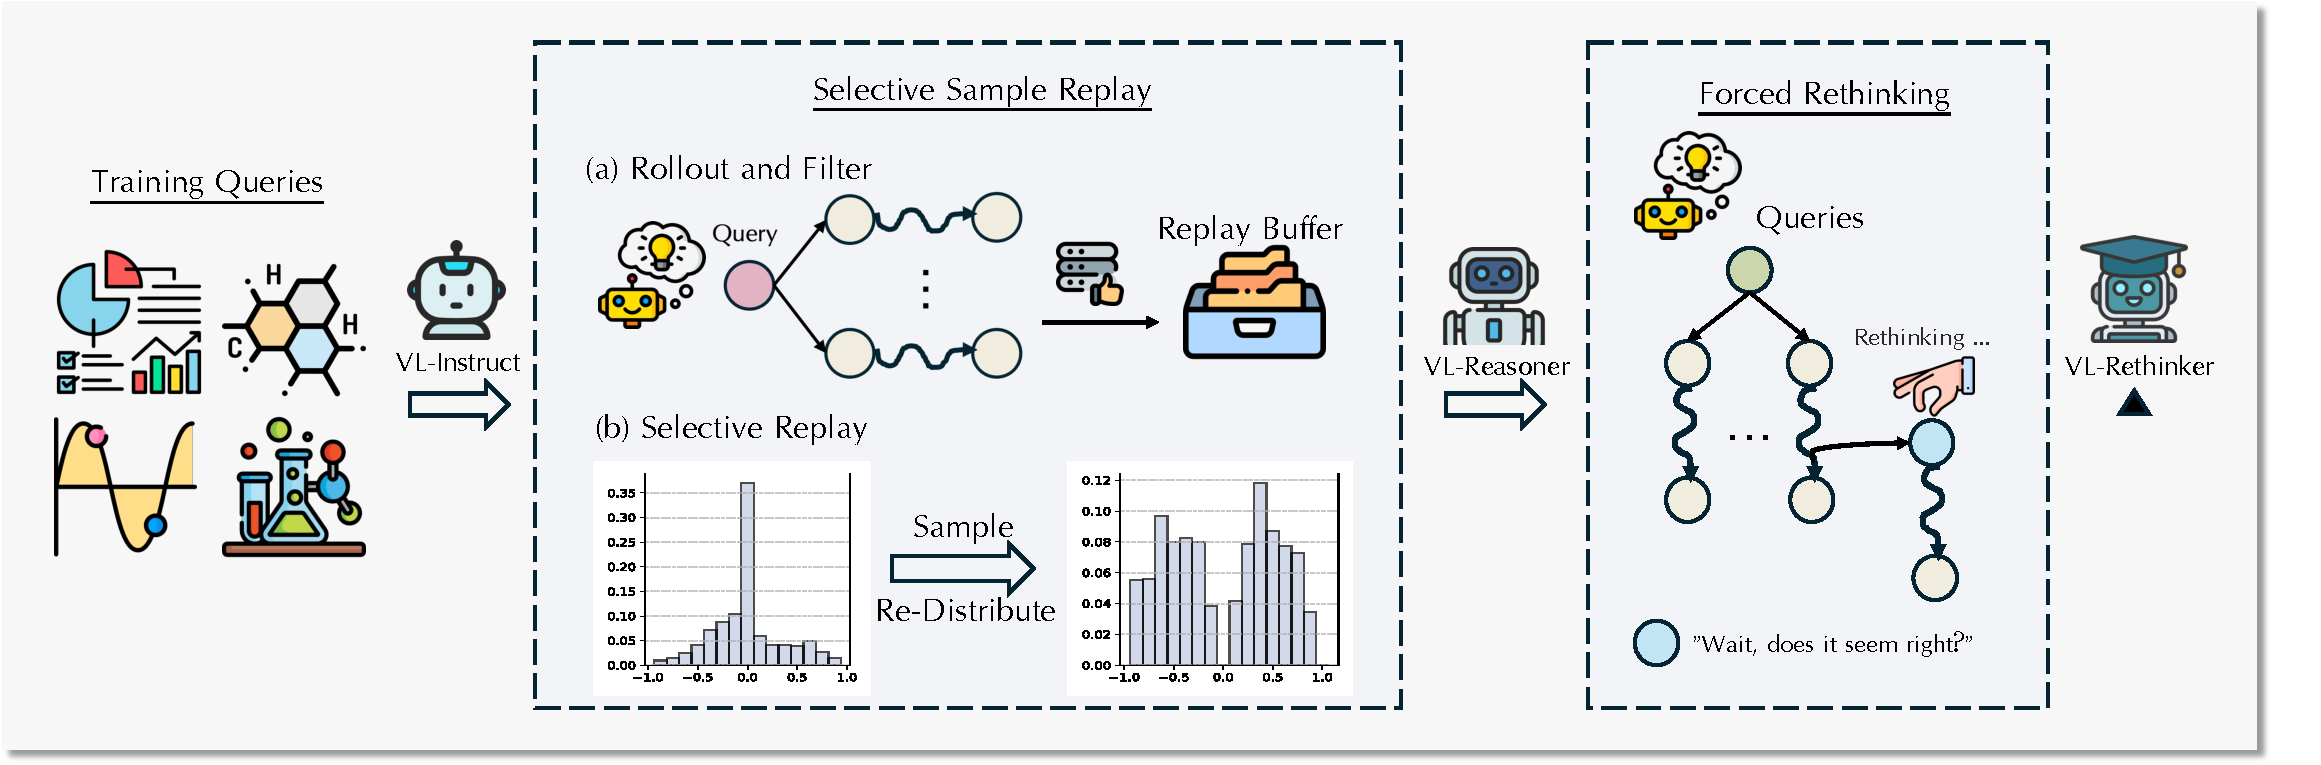
\includegraphics[width=\textwidth]{figures/overview-2.pdf}
\caption{\small \textbf{Method overview.} Starting from an instruction-tuned VLM (VL-Instruct), RL with Selective Sample Replay (SSR) produces VL-Reasoner: (a) rollouts for each query are scored with a binary correctness reward and samples with non-zero advantage are kept in a replay buffer; (b) replay samples from the buffer with priority increasing in $|$advantage$|$, redistributing the training batch away from the spike at zero advantage (left histogram) towards informative samples (right histogram). Forced Rethinking then appends a rethinking trigger (e.g., ``Wait, does it seem right?'') to a fraction of rollouts during RL, yielding \model.}
\label{fig:overview}
\end{figure*}

\begin{table*}[tb]
\centering
\resizebox{\textwidth}{!}{
\begin{tabular}{lccccccc}
\toprule
\textbf{Model}&\multicolumn{3}{c}{\textbf{Math-Related}}&\multicolumn{3}{c}{\textbf{Multi-Discipline}}&\multicolumn{1}{c}{\textbf{Real-World}}\\
\cmidrule(lr){2-4}\cmidrule(lr){5-7}\cmidrule(lr){8-8}
&MathVista&MathVerse&MathVision&MMMU-Pro&MMMU&EMMA&MEGA\\
&testmini&testmini&test&overall&val&full&core\\
\midrule
\multicolumn{8}{c}{\textit{Proprietary Models}}\\
\midrule
OpenAI-o1&73.9&57.0&60.3&62.4&78.2&45.7&56.2\\
OpenAI-GPT-4o&60.0&41.2&30.6&51.9&69.1&32.7&52.7\\
Claude-3.5-Sonnet&67.7&47.8&33.5&51.5&68.3&35.1&52.3\\
Gemini-2.0-Flash&73.4&54.6&41.3&51.7&70.7&33.6&54.1\\
\midrule
\multicolumn{8}{c}{\textit{Open-Source Models}}\\
\midrule
Llama4-Scout-109B&70.7&-&-&\underline{52.2}&69.4&24.6&31.8\\
InternVL-2.5-78B&72.3&51.7&34.9&48.6&61.8&27.1&44.1\\
QvQ-72B&71.4&48.6&35.9&51.5&\textbf{70.3}&32.0&8.8\\
LLaVA-OV-72B&67.5&39.1&30.1&31.0&56.8&23.8&29.7\\
Qwen-2.5-VL-32B&74.7&48.5&\underline{38.4}&49.5&$^\dagger$59.4&31.1&13.3\\
Qwen-2.5-VL-72B&\underline{74.8}&\underline{57.2}&38.1&51.6&$^\dagger$67.0&\underline{34.1}&\underline{49.0}\\
\midrule
\model-32B&78.8&56.9&40.5&50.6&65.6&37.9&19.9\\
\model-72B&\textbf{80.4}&\textbf{63.5}&\textbf{44.9}&\textbf{55.9}&68.8&\textbf{38.5}&\textbf{51.3}\\
\rowcolor{cyan!20}
$\Delta$ (\model-72B $-$ best other open)&+5.6&+6.3&+6.5&+3.7&$-$1.5&+4.4&+2.3\\
\bottomrule
\end{tabular}
}
\caption{\small \textbf{Comparison of \model-72B with proprietary and open-source models.} Accuracy (\%) on each benchmark split. Within the open-source block, \textbf{bold} marks the best score and \underline{underline} the best score of another open-source model, the reference for the $\Delta$ row (on MMMU, QvQ-72B is both). Proprietary models are listed for reference and are not marked; OpenAI-o1 remains ahead on MathVision, MMMU-Pro, MMMU, EMMA and MEGA. $^\dagger$: reproduced with our evaluation protocol; ``-'': not reported.}
\label{table:main_results}
\end{table*}

\begin{table*}[tb]
\centering
\resizebox{\textwidth}{!}{
\begin{tabular}{lccccccc}
\toprule
\textbf{Model}&\multicolumn{3}{c}{\textbf{Math-Related}}&\multicolumn{3}{c}{\textbf{Multi-Discipline}}&\multicolumn{1}{c}{\textbf{Real-World}}\\
\cmidrule(lr){2-4}\cmidrule(lr){5-7}\cmidrule(lr){8-8}
&MathVista&MathVerse&MathVision&MMMU-Pro&MMMU&EMMA&MEGA\\
&testmini&testmini&test&overall&val&full&core\\
\midrule
\multicolumn{8}{c}{\textit{General Vision-Language Models}}\\
\midrule
InternVL2-8B&58.3&-&17.4&29.0&51.2&19.8&26.0\\
InternVL2.5-8B&64.4&39.5&19.7&34.3&\underline{56.0}&-&30.4\\
Qwen2-VL-7B&58.2&-&16.3&30.5&54.1&20.2&34.8\\
Qwen2.5-VL-7B&68.2&46.3&25.1&36.9&$^\dagger$54.3&21.5&\underline{35.0}\\
LLaVA-OV-7B&63.2&26.2&-&24.1&48.8&18.3&22.9\\
Kimi-VL-16B&68.7&44.9&21.4&-&$^\dagger$55.7&-&-\\
\midrule
\multicolumn{8}{c}{\textit{Vision-Language Reasoning Models}}\\
\midrule
MM-Eureka-8B (InternVL)&67.1&40.4&22.2&27.8&49.2&-&-\\
MM-Eureka-7B (Qwen)&\underline{73.0}&\underline{50.3}&26.9&-&-&-&-\\
R1-VL-7B&63.5&40.0&24.7&7.8&44.5&8.3&29.9\\
R1-Onevision-7B&64.1&46.4&\underline{29.9}&21.6&-&20.8&27.1\\
OpenVLThinker-7B&70.2&47.9&25.3&\underline{37.3}&52.5&\underline{26.6}&12.0\\
\midrule
\model-7B&\textbf{74.9}&\textbf{54.2}&\textbf{32.3}&\textbf{41.7}&\textbf{56.7}&\textbf{29.7}&\textbf{37.2}\\
\rowcolor{cyan!20}
$\Delta$ (\model-7B $-$ best other)&+1.9&+3.9&+2.4&+4.4&+0.7&+3.1&+2.2\\
\bottomrule
\end{tabular}
}
\caption{\small \textbf{Comparison of \model-7B with general and reasoning vision-language models of similar size.} Accuracy (\%) on each benchmark split. \textbf{Bold}: best score; \underline{underline}: best score of any other listed model, the reference for the $\Delta$ row. $^\dagger$: reproduced with our evaluation protocol; ``-'': not reported.}
\label{table:7b_results}
\end{table*}

\begin{table*}[tb]
\centering
\resizebox{\textwidth}{!}{
\begin{tabular}{lcccccccc}
\toprule
\textbf{Model}&RL algorithm&Forced Rethinking&Training data&MathVision&MathVista&MathVerse&MMMU-Pro&EMMA\\
\midrule
\model-7B&GRPO-SSR&\ding{51}&16K&\textbf{32.3}&\textbf{74.9}&\textbf{54.2}&\textbf{41.7}&\textbf{29.7}\\
\midrule
VL-Reasoner-7B (w/o Forced Rethinking)&GRPO-SSR&\ding{55}&16K&29.8&72.4&53.2&40.9&29.5\\
\quad $-$ SSR (GRPO-Filter)&GRPO-Filter&\ding{55}&16K&28.5&72.0&50.0&40.0&26.9\\
\quad $-$ SSR $-$ Filter (vanilla GRPO)&GRPO&\ding{55}&16K&26.0&70.9&51.4&38.8&26.2\\
\midrule
\quad $-$ text-only data&GRPO-SSR&\ding{55}&13K&29.1&73.5&53.5&41.1&28.7\\
\quad $-$ science and text-only data&GRPO-SSR&\ding{55}&11K&28.0&71.6&50.3&39.7&28.0\\
\bottomrule
\end{tabular}
}
\caption{\small \textbf{Ablation of Forced Rethinking, Selective Sample Replay (SSR) and the training-data mix} at 7B scale. Accuracy (\%) on MathVision test, MathVista testmini, MathVerse testmini, MMMU-Pro overall and EMMA full. Indented rows each remove the named component(s) from VL-Reasoner-7B, the SSR-trained model before Forced Rethinking. GRPO-Filter discards zero-advantage samples and refills the batch uniformly from the current step's non-zero-advantage samples, without SSR's cross-step buffer and $|$advantage$|$-prioritised replay. \textbf{Bold}: best per column.}
\label{table:ablation_results}
\end{table*}

\begin{figure*}[!tbp]
\centering
\begin{subfigure}[b]{0.85\textwidth}
\centering
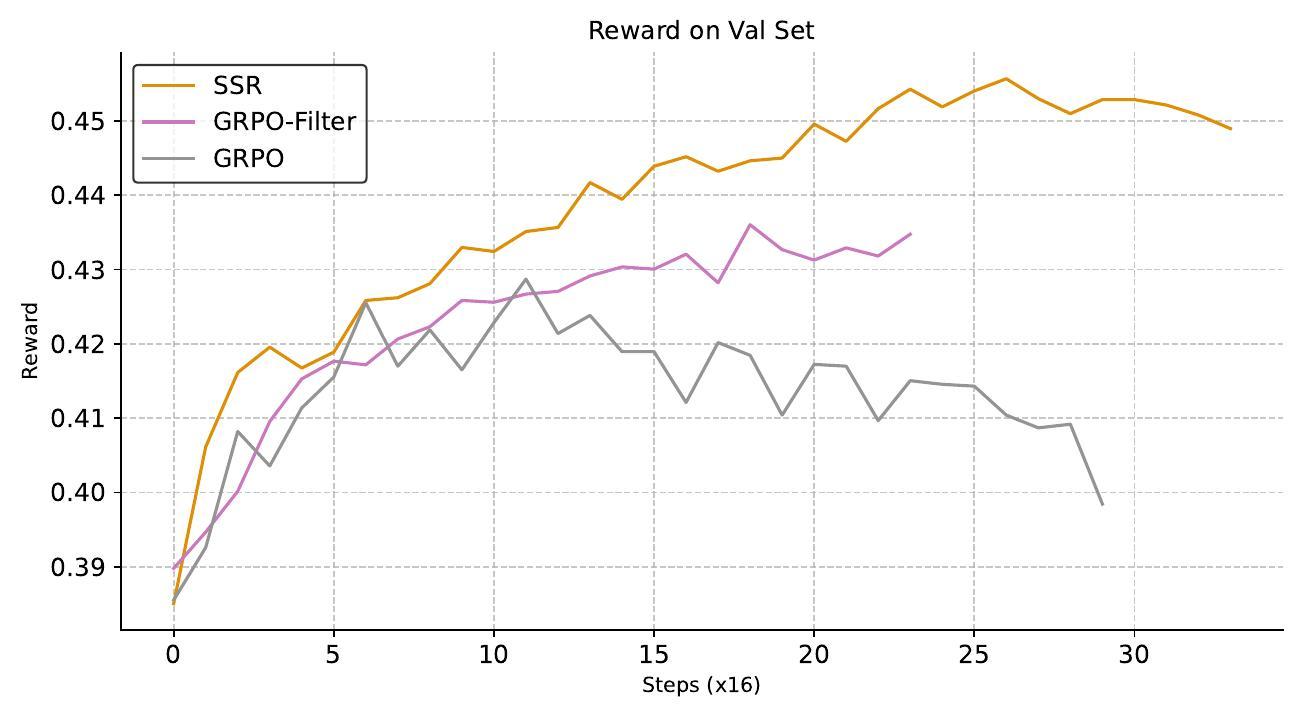
\includegraphics[width=\linewidth]{figures/ssr_eval_curve.jpg}
\caption{Validation reward during training.}
\label{fig:ssr_eval_curve}
\end{subfigure}
\par\smallskip
\begin{subfigure}[b]{\textwidth}
\centering
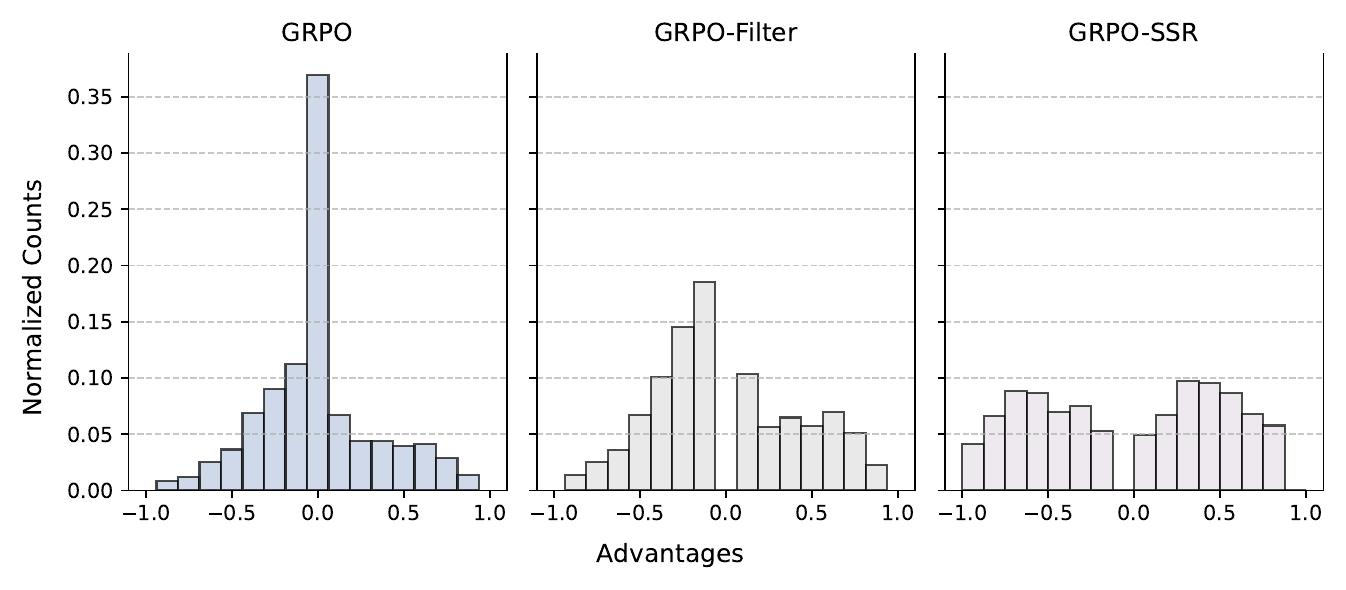
\includegraphics[width=\linewidth]{figures/adv_histogram.jpg}
\caption{Distribution of advantages in training batches.}
\label{fig:adv_histogram}
\end{subfigure}
\caption{\small \textbf{Training dynamics of GRPO, GRPO-Filter and GRPO-SSR.} (a) Mean reward (accuracy) on the held-out validation set; the x-axis counts logged points, one every 16 training steps. Vanilla GRPO peaks at about 0.43 near point 11 ($\approx$180 steps), then declines to about 0.40 by point 29. GRPO-Filter keeps improving to about 0.435 over its shorter run (23 points, $\approx$370 steps). GRPO-SSR improves fastest and reaches about 0.455 around points 23--26 ($\approx$370--420 steps). Each curve is a single run. (b) Normalised histograms of the advantages of the samples used for policy updates. Under GRPO, about 37\% of samples sit in the bin at zero advantage. Filtering removes exact zeros but leaves the mass concentrated at small $|$advantage$|$. SSR's $|$advantage$|$-prioritised replay shifts the mass towards $|$advantage$|\approx 0.3$--$0.9$.}
\label{fig:training_dynamics}
\end{figure*}

\begin{figure*}[tb]
\centering
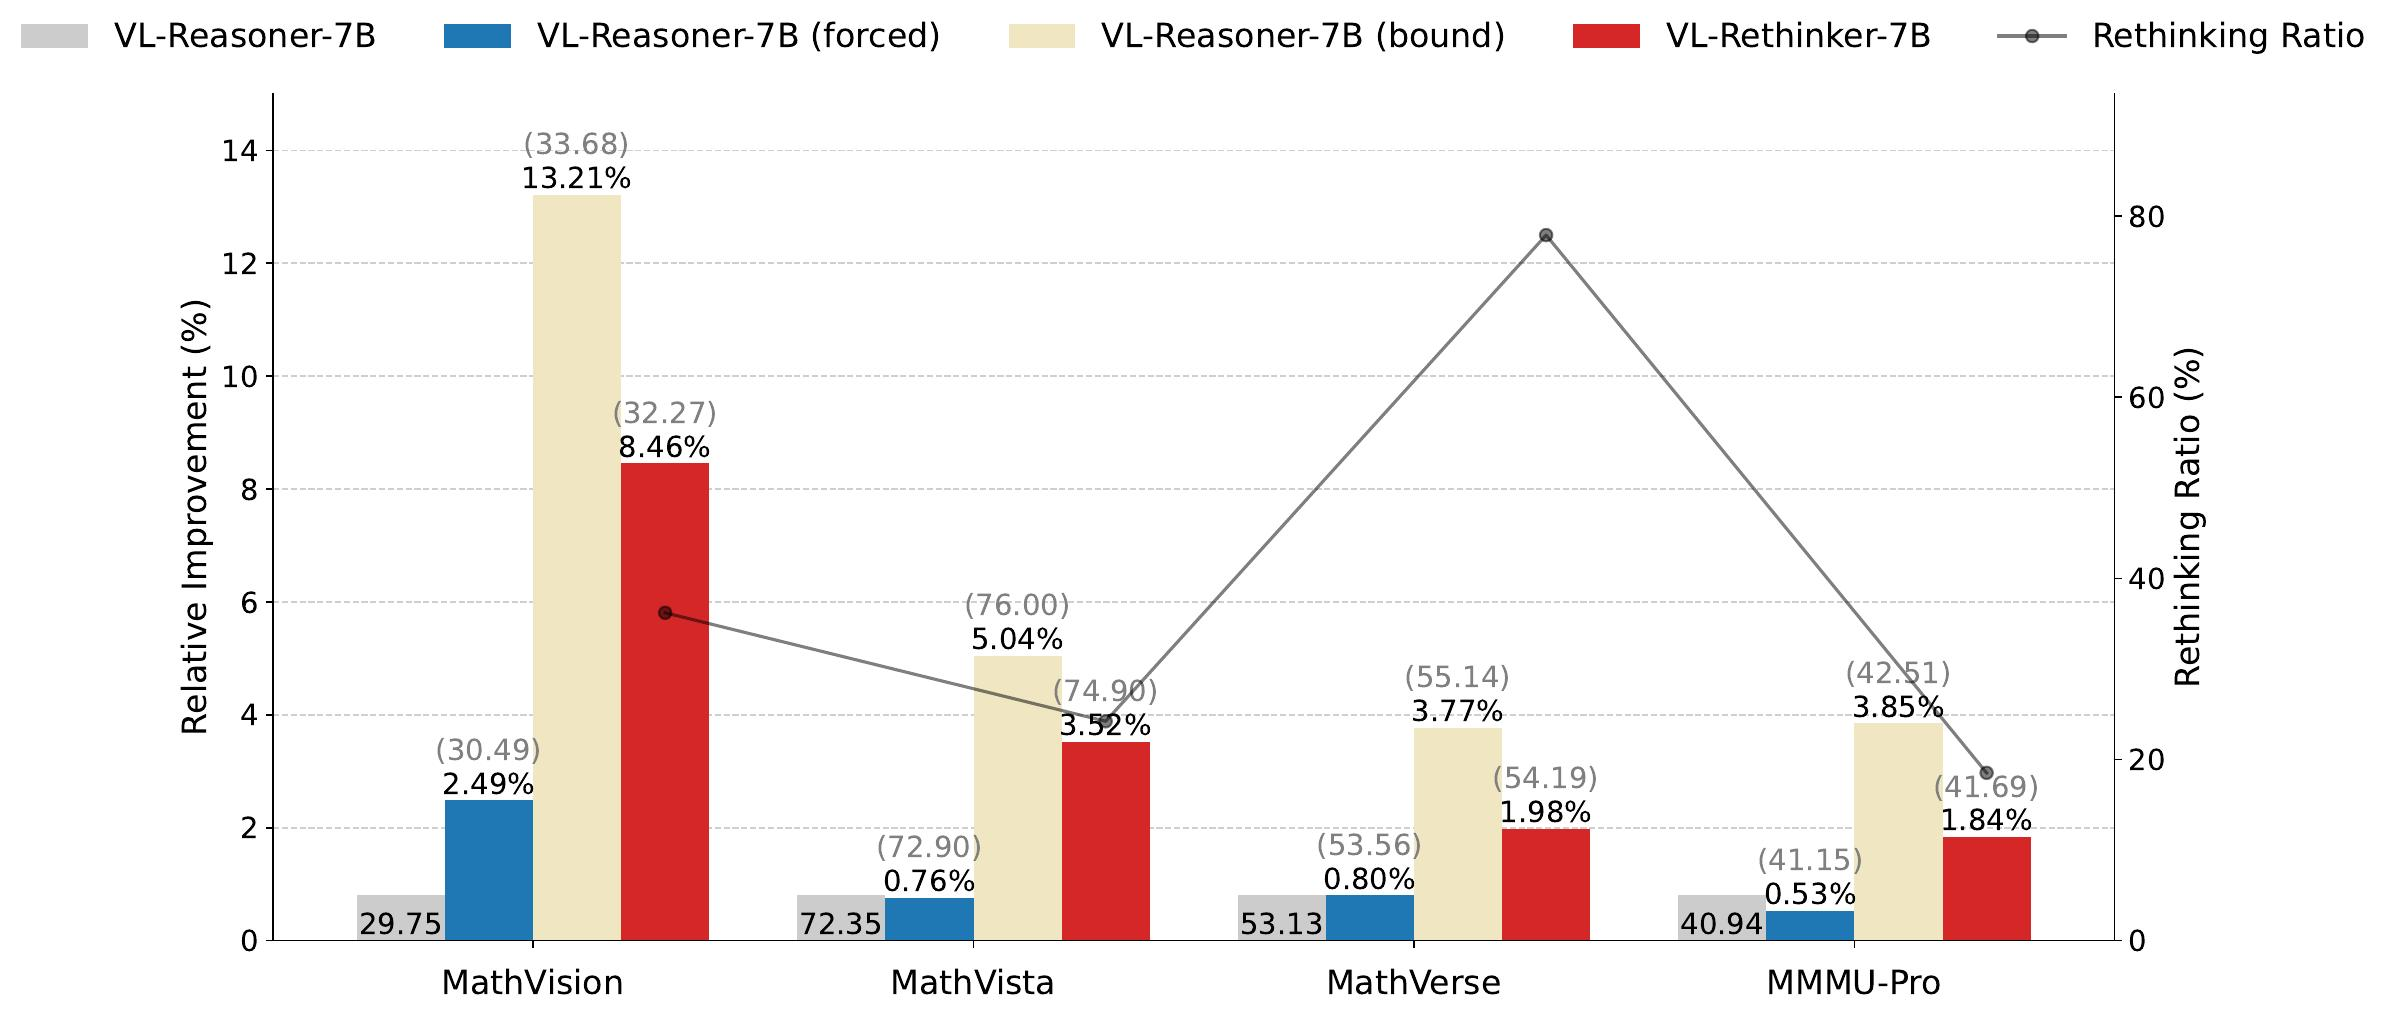
\includegraphics[width=\textwidth]{figures/foret_ablation.jpg}
\caption{\small \textbf{Relative improvement with different rethinking strategies at 7B.} Bars (left axis) give the relative improvement (\%) over VL-Reasoner-7B, the SSR-trained model without Forced Rethinking (gray, its accuracy printed at the bar base). Absolute accuracies are in parentheses. Blue: VL-Reasoner-7B forced to rethink at test time. Beige: an oracle upper bound of test-time rethinking for VL-Reasoner-7B, in which the rethought answer replaces the original only when it is correct. Red: \model-7B, trained with Forced Rethinking. The line (right axis) gives the fraction of \model-7B responses that contain a self-reflection phrase (e.g., ``wait''). Test-time forcing alone gives small gains (0.5--2.5\%), whereas training with Forced Rethinking gives 1.8--8.5\%, with the largest gain on MathVision. \model-7B rethinks selectively rather than uniformly: about 78\% of responses on MathVerse, 36\% on MathVision, and about 24\% and 18\% on MathVista and MMMU-Pro.}
\label{fig:foret_ablation}
\end{figure*}

% Wrapped beside the text when the preamble loads wrapfig (\input it between paragraphs);
% otherwise an ordinary float of the same width.
\ifdefined\wrapfigure
\begin{wrapfigure}{r}{0.5\linewidth}
\vspace{-1em}
\centering
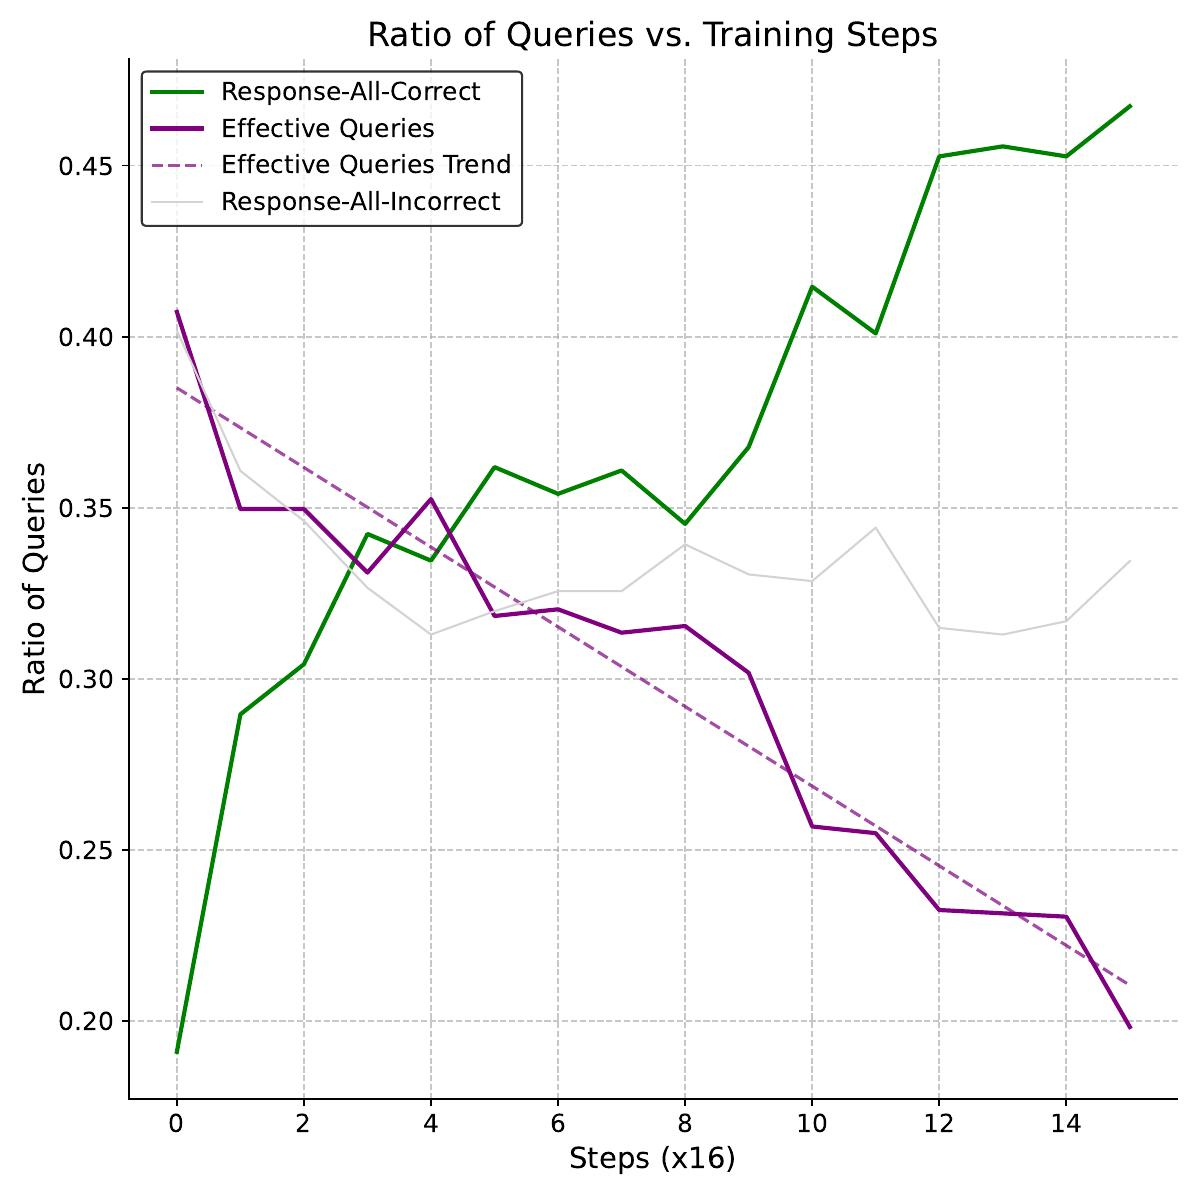
\includegraphics[width=\linewidth]{figures/vanishing_adv.jpg}
\caption{\small \textbf{Vanishing advantages in GRPO training.} Fraction of training queries per step (x-axis: logged points, one every 16 training steps) whose rollouts are all correct (green), all incorrect (gray) or mixed (``effective queries'', purple; dashed: linear trend). Only mixed groups receive a non-zero group-normalised advantage. Over training the effective fraction falls from about 0.41 to 0.20, while the all-correct fraction rises from about 0.19 to 0.47.}
\label{fig:vanishing_adv}
\vspace{-1em}
\end{wrapfigure}
\else
\begin{figure}[tb]
\centering
\begin{minipage}{0.5\linewidth}
\centering
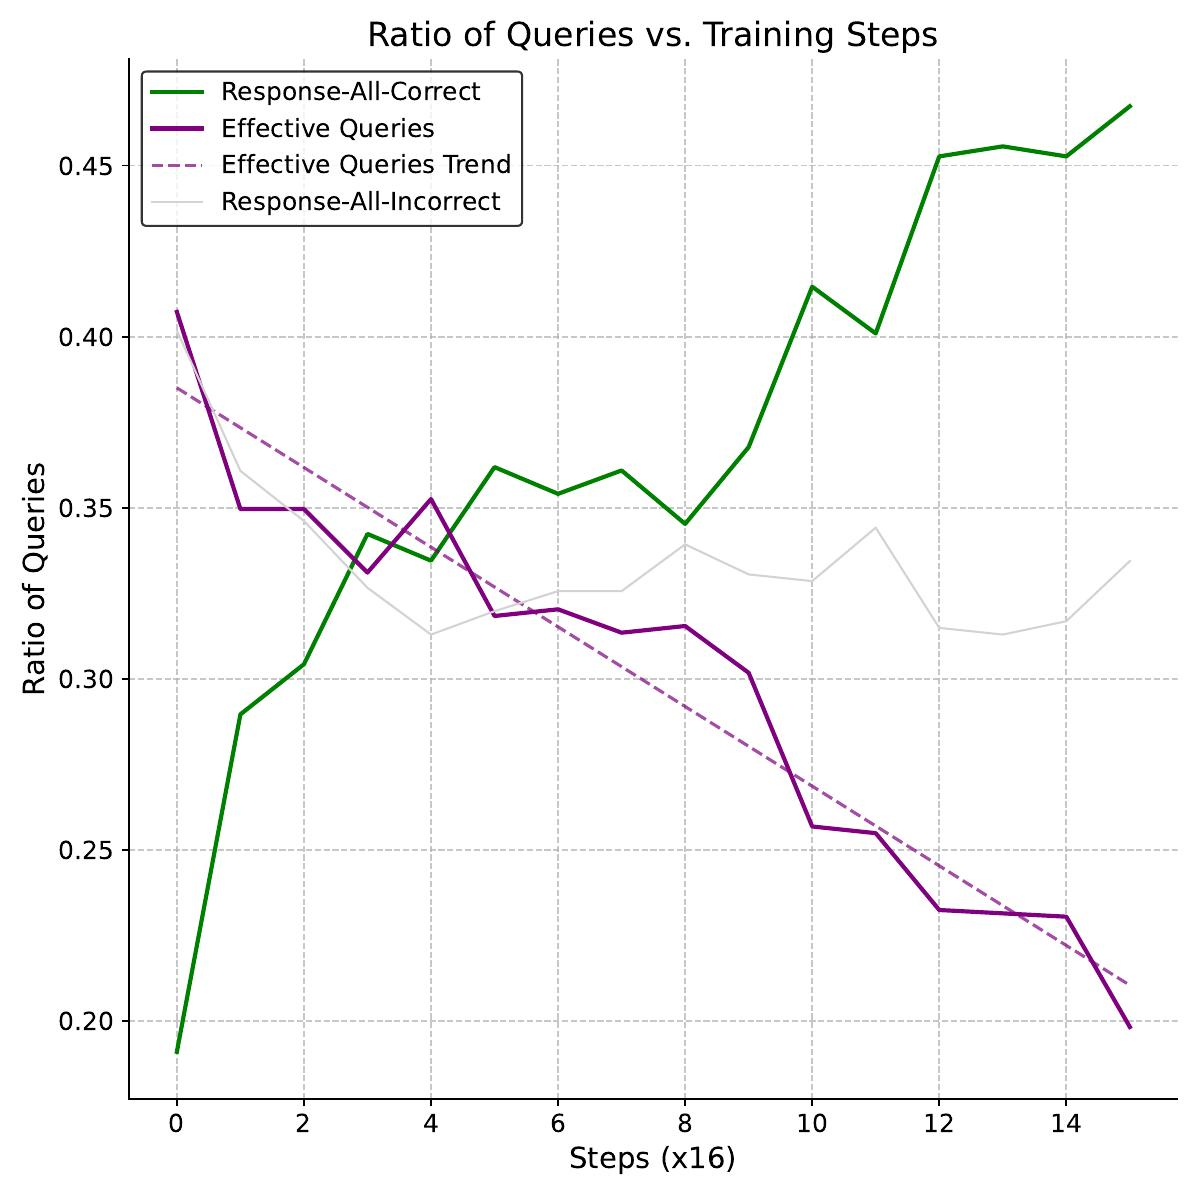
\includegraphics[width=\linewidth]{figures/vanishing_adv.jpg}
\caption{\small \textbf{Vanishing advantages in GRPO training.} Fraction of training queries per step (x-axis: logged points, one every 16 training steps) whose rollouts are all correct (green), all incorrect (gray) or mixed (``effective queries'', purple; dashed: linear trend). Only mixed groups receive a non-zero group-normalised advantage. Over training the effective fraction falls from about 0.41 to 0.20, while the all-correct fraction rises from about 0.19 to 0.47.}
\label{fig:vanishing_adv}
\end{minipage}
\end{figure}
\fi

\begin{figure}[tb]
\centering
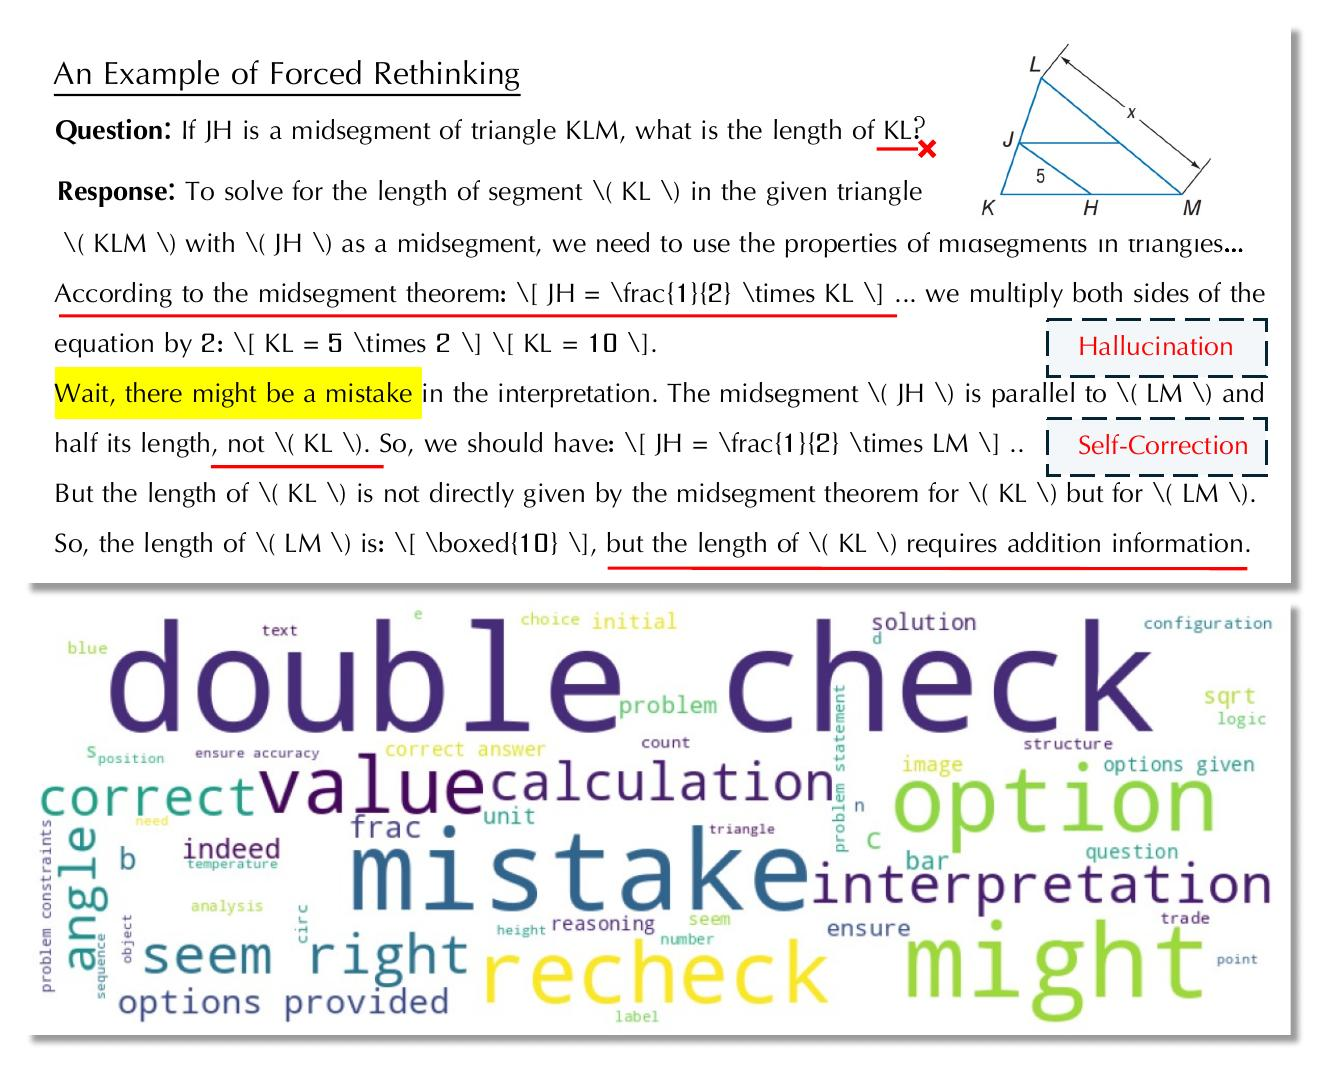
\includegraphics[width=\linewidth,height=0.3\textheight,keepaspectratio]{figures/rethinking.jpg}
\caption{\small \textbf{Forced Rethinking in practice.} \emph{Top:} a response from training with Forced Rethinking. The initial reasoning misapplies the midsegment theorem (JH $=\tfrac12$KL, a hallucinated relation). After the appended trigger ``Wait, there might be a mistake'', the model notices that JH is parallel to and half of LM, not KL, and revises its conclusion (self-correction). \emph{Bottom:} word cloud of the rethinking segments, dominated by verification and correction phrases (``double check'', ``mistake'', ``recheck'', ``might'', ``seem right'').}
\label{fig:rethinking}
\end{figure}

Refs: \ref{fig:teaser} \ref{fig:overview} \ref{table:main_results} \ref{table:7b_results} \ref{table:ablation_results} \ref{fig:training_dynamics} \ref{fig:ssr_eval_curve} \ref{fig:adv_histogram} \ref{fig:foret_ablation} \ref{fig:vanishing_adv} \ref{fig:rethinking}
\clearpage
\end{document}
